\documentclass{article}
\usepackage{graphicx} % Required for inserting images
\usepackage{float}
\usepackage[T1]{fontenc}
\usepackage{amsmath}
\usepackage[margin=1in]{geometry}
\usepackage{booktabs}
\usepackage{tabularx}
\usepackage[hidelinks]{hyperref}

\title{Sizing the always-on 25-delta put to a 35\% stress budget passes, but much of the gain comes from selling big into vol spikes}
\author{Experiment report \textperiodcentered{} L/S Gamma Desk, QUANTT}
\date{2026-10-22}

\begin{document}

\maketitle

\textbf{Question:} If the always-on 25-delta short put (\texttt{always25}) is sized at every entry to the most contracts whose loss in a one-day 20\% SPY drop, with implied vol at 60\%, stays within 35\% of capital, does it beat one-contract \texttt{always25} at 1x and 2x spreads, over the full window and in each half, with a maximum drawdown within that \$87,500 budget? How do daily hedging, a Whalley-Wilmott band and no hedge compare at the same budget, and should share hedges move to IBKR Tiered pricing?

\textbf{Method:}

\begin{itemize}

\item Pre-registered backtest: the research switches were committed in 424f8d6 and the hypothesis card in a515c6d, before any run.

\item The live paper rules (\texttt{configs/\allowbreak{}paper.\allowbreak{}toml}) are replayed on R2 replay snapshots v1 (config\_hash b040760187f0) over the development window 2014-06-02 to 2024-12-31. The hold-out (2025-01-01 to 2026-07-10) was not used.

\item \textbf{All variants:} the \texttt{always25} book.

\begin{itemize}

\item The VRP signal is ignored (\texttt{short\_\allowbreak{}band = long\_\allowbreak{}band = -\allowbreak{}inf}), so the book is always short and rolls at the 7-DTE time exit.

\item The 1x-credit stop, 50\% profit-take and 1-day cool-off are as live.

\item New switch: \texttt{stress\_\allowbreak{}budget = 0.\allowbreak{}35}, with \texttt{stress\_\allowbreak{}drop = 0.\allowbreak{}20} and \texttt{stress\_\allowbreak{}vol = 0.\allowbreak{}60}.

\end{itemize}

\item \textbf{Sizing:} at each entry, contracts = the largest n whose scenario loss fits the budget.

\begin{itemize}

\item The scenario prices the put at spot \ensuremath{-}20\% and IV = max(60\%, its IV), using Black-Scholes.

\item The hedge offsets the put's delta. The shares a hedge band can leave open count as unhedged.

\end{itemize}

\item \textbf{Variants:}

\begin{itemize}

\item \texttt{hedged} (primary): the daily 10-share hedge, as \texttt{always25}.

\item \texttt{banded}: \texttt{min\_\allowbreak{}shares = 1} and \texttt{ww\_\allowbreak{}band = 30}. It re-hedges fully once the drift reaches 30 \ensuremath{\times} \ensuremath{\surd}(book gamma in shares per \$1).

\item \texttt{unhedged}: \texttt{min\_\allowbreak{}shares = 1e9}.

\end{itemize}

\item \textbf{Comparison:} the registered \texttt{2026-\allowbreak{}10-\allowbreak{}17-\allowbreak{}always-\allowbreak{}short/\allowbreak{}always25} runs, reused, at the same spread multiple.

\item \textbf{Runs and costs:} every variant at 1x and 2x spreads. \$0.65 per contract and \$0.005 per share, with a \$1 minimum per order. Exits and hedges run once a day at 10:15 ET.

\item \textbf{Tiered vs Fixed:} answered by re-pricing every logged hedge order; no extra runs were needed.

\end{itemize}

This report was written by Claude at the PM's request.

\section{Result vs the pass bar}

Every check had to hold at 1x and 2x spreads. P\&L and drawdown are in USD on \$250k of capital. The reference \texttt{always25} trades one contract; the sized books trade 8-100.

\begin{center}\small
\begin{tabularx}{\linewidth}{>{\raggedright\arraybackslash}X l l l l l}
\toprule
\textbf{Check (\texttt{hedged} vs \texttt{always25})} & \textbf{1x value} & \textbf{1x bar} & \textbf{2x value} & \textbf{2x bar} & \textbf{Result} \\
\midrule
Net P\&L, full window & \$121,482 & > \$1,316 & \$101,172 & > \$862 & pass \\
Net P\&L, 2014-06 to 2019-12 & \$49,132 & > \$553 & \$42,687 & > \$371 & pass \\
Net P\&L, 2020-01 to 2024-12 & \$72,350 & > \$763 & \$58,485 & > \$491 & pass \\
Net P\&L above zero, full window & \$121,482 & > \$0 & \$101,172 & > \$0 & pass \\
Max drawdown within the budget & \$70,362 & \ensuremath{\leq} \$87,500 & \$75,488 & \ensuremath{\leq} \$87,500 & pass \\
Round trips (floor 30) & 182 & \ensuremath{\geq} 30 &  &  & met \\
\bottomrule
\end{tabularx}
\end{center}

\textbf{Verdict: passed (in-sample).} Sized to the 35\% budget, the hedged always-on put made about \$121k at 1x and \$101k at 2x over 10.6 years, and its drawdown stayed inside the budget, using 80\% of it at 1x and 86\% at 2x. About half of that P\&L came from two entries at the March 2020 volatility peak, where the rule sold 100 and 71 contracts. At those IVs the 25-delta put sits far out of the money, and the scenario's 60\% IV adds little or no further vol shock.

\subsection{Full-window numbers (not part of the bar)}

All values are at 1x spreads unless marked.

\begin{center}\small
\begin{tabularx}{\linewidth}{l >{\raggedright\arraybackslash}X l l l l}
\toprule
\textbf{} & \textbf{baseline} & \textbf{always25} & \textbf{hedged} & \textbf{banded} & \textbf{unhedged} \\
\midrule
Net P\&L & \ensuremath{-}\$2,060 & \$1,316 & \$121,482 & \$114,559 & \$253,839 \\
Net P\&L, 2x & \ensuremath{-}\$4,122 & \$862 & \$101,172 & \$96,288 & \$239,831 \\
Sharpe 1x/\allowbreak{}2x & \ensuremath{-}0.36 /\allowbreak{} \ensuremath{-}0.68 & 0.19 /\allowbreak{} 0.12 & 0.52 /\allowbreak{} 0.43 & 0.61 /\allowbreak{} 0.51 & 0.80 /\allowbreak{} 0.75 \\
Max drawdown & \$3,027 & \$2,041 & \$70,362 & \$48,744 & \$58,469 \\
Worst day & \ensuremath{-}\$468 & \ensuremath{-}\$677 & \ensuremath{-}\$19,791 & \ensuremath{-}\$21,966 & \ensuremath{-}\$29,114 \\
ES 5\%, daily & \ensuremath{-}\$96 & \ensuremath{-}\$121 & \ensuremath{-}\$3,016 & \ensuremath{-}\$2,586 & \ensuremath{-}\$5,195 \\
Round trips & 131 & 187 & 182 & 187 & 412 \\
Contracts & 131 & 187 & 4,617 & 4,110 & 7,154 \\
Option fees & \$262 & \$372 & \$5,955 & \$5,324 & \$9,300 \\
Hedge fees & \$914 & \$609 & \$2,868 & \$1,040 & \$0 \\
2023-24 P\&L & \ensuremath{-}\$674 & \ensuremath{-}\$475 & \$4,969 & \$10,018 & \$72,984 \\
\bottomrule
\end{tabularx}
\end{center}

\section{Charts}

\begin{figure}[H]\centering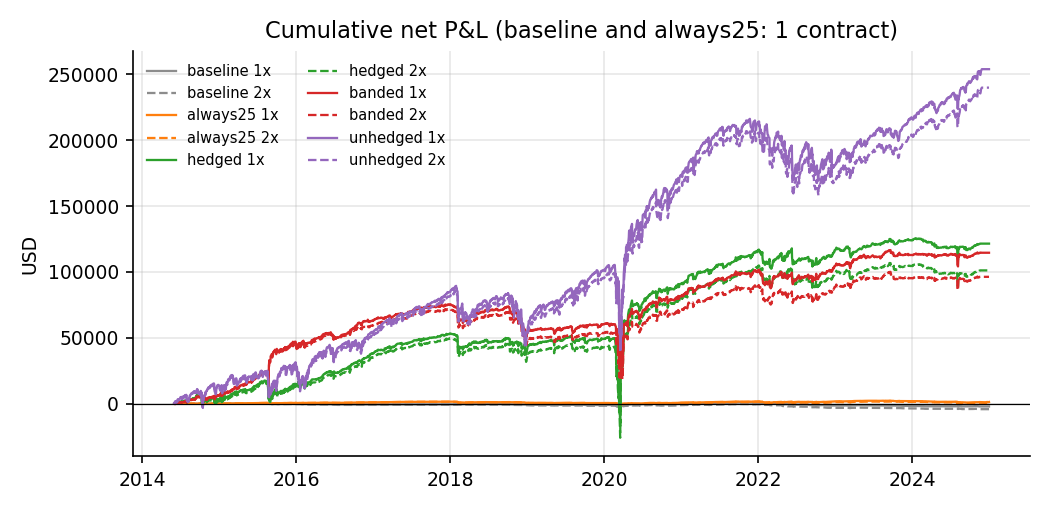
\includegraphics[width=0.92\linewidth]{figures/cum_pnl.png}\caption{Cumulative net P\&L, 1x solid and 2x dashed; baseline grey, always25 orange (both one contract)}\end{figure}

The sized books dwarf the one-contract lines. The hedged book (green) climbs steadily to 2018, stalls until early 2020, then drops about \$67k in four weeks and recovers it within a week in March 2020. The banded book (red) takes a step up in August 2015. The unhedged book (purple) moves with the stock market, including 2018 and 2022.

\begin{figure}[H]\centering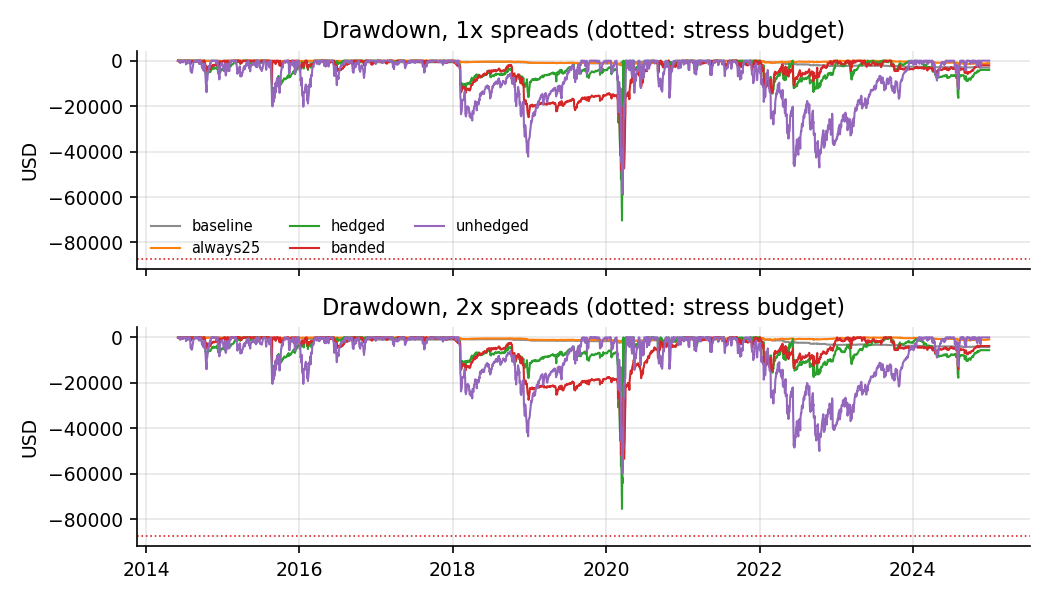
\includegraphics[width=0.92\linewidth]{figures/drawdown.png}\caption{Drawdown at 1x and 2x spreads; the dotted line is the \$87,500 stress budget}\end{figure}

Every sized book stays above the budget line. The deepest point for all three is March 2020: \$70.4k for hedged, \$48.7k for banded and \$58.5k for unhedged at 1x. The unhedged book also spends 2022 in a drawdown of up to \$47k.

\begin{figure}[H]\centering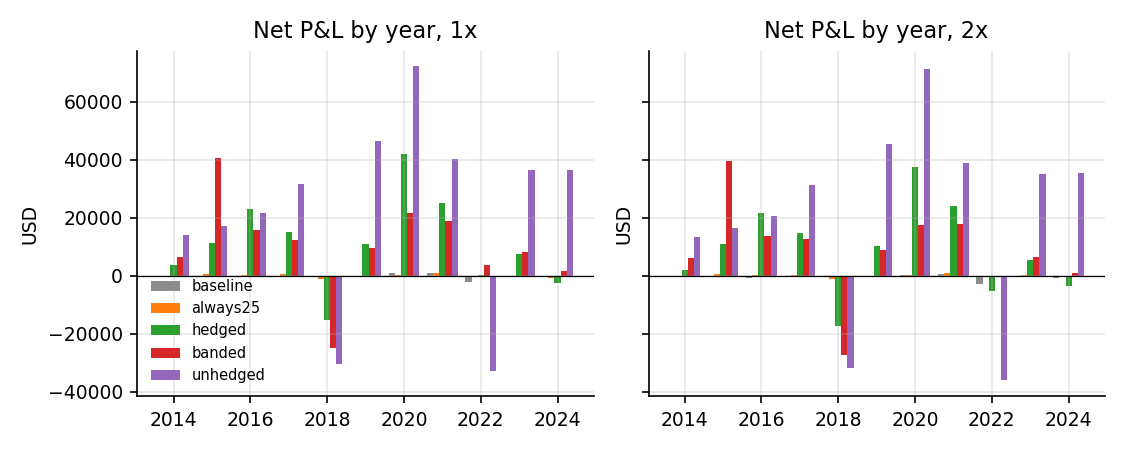
\includegraphics[width=0.92\linewidth]{figures/yearly.png}\caption{Net P\&L by year}\end{figure}

The hedged book loses in 2018 (\ensuremath{-}\$15.2k: February, October and December) and 2024 (\ensuremath{-}\$2.6k), and earns \$42.0k in 2020. From 2022 its yearly P\&L is small: +\$0.4k, +\$7.6k and \ensuremath{-}\$2.6k. The unhedged book has the largest swings: \ensuremath{-}\$30.4k in 2018 and \ensuremath{-}\$32.8k in 2022.

\begin{figure}[H]\centering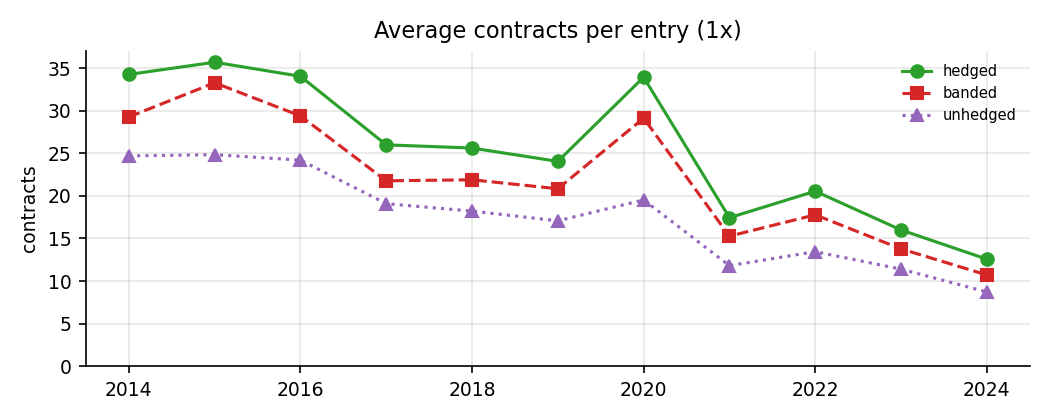
\includegraphics[width=0.92\linewidth]{figures/contracts.png}\caption{Average contracts per entry, 1x}\end{figure}

Contracts per entry fall from about 34 (hedged) in 2014-2016 to 13 in 2024. SPY roughly tripled, so the same stress loss buys fewer contracts and notional stays near \$700k (median, hedged). The 2020 average is lifted by the March entries. On the 2026-10-21 chain the rule gives 8 contracts hedged, 7 banded and 6 unhedged (desk calculation).

\begin{figure}[H]\centering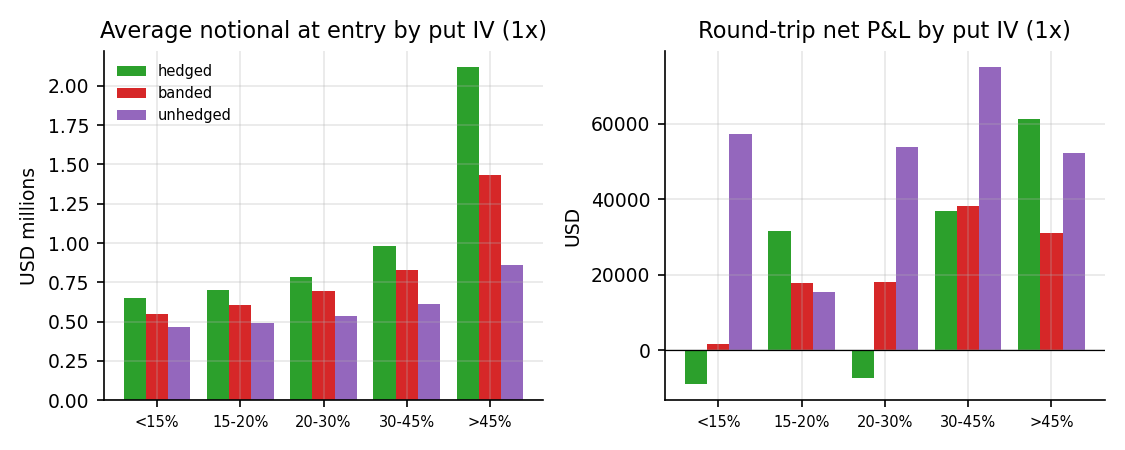
\includegraphics[width=0.92\linewidth]{figures/iv_buckets.png}\caption{Average notional at entry and round-trip net P\&L, by the put's implied vol at entry, 1x}\end{figure}

This chart shows where the money came from. Notional rises with IV: the correlation between IV and notional at entry is 0.90 hedged, 0.95 banded and 0.96 unhedged.

For the hedged book, the 72 entries below 15\% IV lost \$9.1k and the 50 between 20\% and 30\% lost \$7.5k. The two entries above 45\% IV, both in March 2020 at about 86 contracts on average, made \$61.3k of the book's \$113.2k round-trip net. The banded book earned in every IV bucket.

\begin{figure}[H]\centering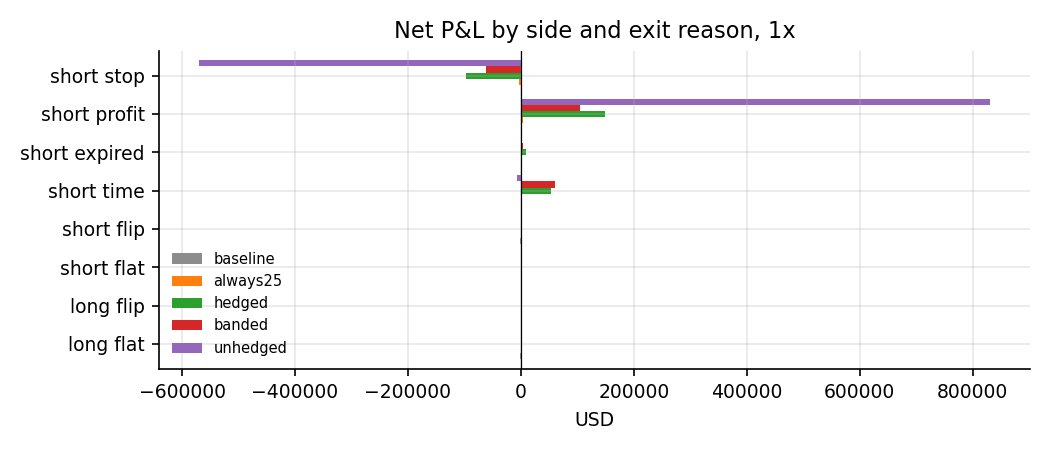
\includegraphics[width=0.92\linewidth]{figures/by_reason.png}\caption{Net P\&L by side and exit reason, 1x}\end{figure}

The hedged and banded books earn on profit-takes and time exits and lose on stops. The unhedged book is different. Its option-only P\&L hits the 50\% profit-take quickly in rising markets and the stop in falling ones: 318 profit-takes and 88 stops against 6 time exits, with an average hold of 9 days against 21.

\begin{figure}[H]\centering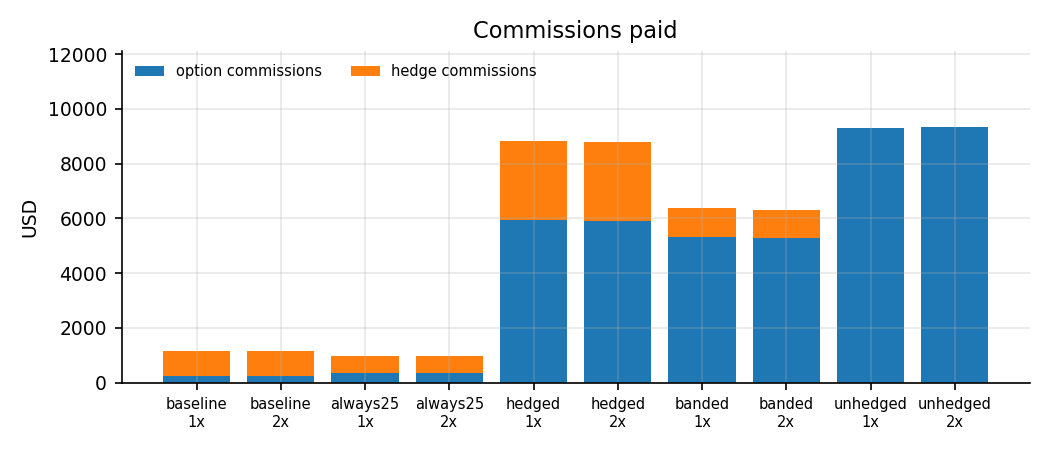
\includegraphics[width=0.92\linewidth]{figures/fees.png}\caption{Commissions paid}\end{figure}

Size dilutes the \$1 minimums. Commissions per contract fall from \$5.25 for \texttt{always25} to \$1.91 hedged, \$1.55 banded and \$1.30 unhedged. The band cuts hedge orders from 2,317 to 639 and hedge commissions from \$2,868 to \$1,040.

\begin{figure}[H]\centering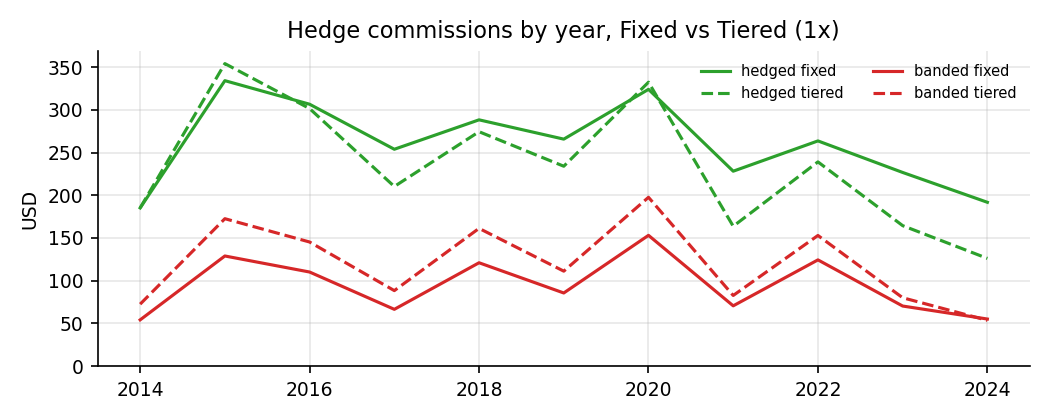
\includegraphics[width=0.92\linewidth]{figures/tiered.png}\caption{Hedge commissions by year under IBKR Fixed and Tiered, 1x}\end{figure}

Tiered is cheaper for orders under about 150 shares and dearer above that. The hedged book's orders shrank as SPY rose: a median of 56 shares in 2023-2024, 83\% of them under 149. Its Tiered cost there is \$291 against \$418 under Fixed, 31\% lower, and \$2,585 against \$2,868 over the full window. The banded book trades fewer, larger orders (median 260 shares), so Tiered would cost it more: \$1,318 against \$1,040.

\begin{figure}[H]\centering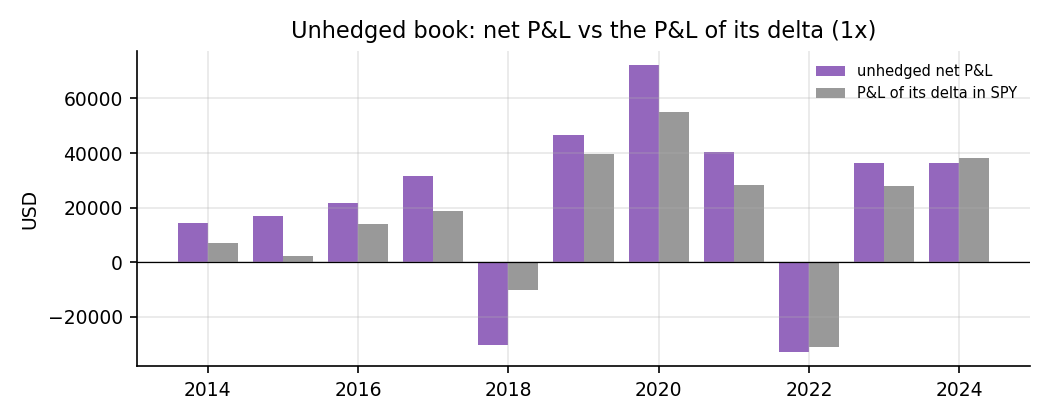
\includegraphics[width=0.92\linewidth]{figures/beta.png}\caption{Unhedged book: net P\&L against the P\&L of holding its delta in SPY, 1x}\end{figure}

Holding the unhedged book's option delta in SPY between decisions would have made \$190.4k. That is 75\% of its \$253.8k net. Without it, the unhedged book earned about \$63.5k at 1x and \$49.0k at 2x, about half of the hedged book's P\&L for a similar stress budget.

\section{Analysis}

\textbf{Size alone explains less than half of the gain.} The sized books average 9-36 contracts per entry, depending on the year and the variant. Net P\&L per contract sold rose from \$7.03 (\texttt{always25}) to \$26.31 (hedged), and cheaper commissions explain \$3.34 of that. At \texttt{always25}'s \$7.03 plus that saving, the hedged book's 4,617 contracts would have made about \$48k of its \$121.5k. Most of the other \$74k comes from the two March 2020 trades (below), and some from different exits.

The paths also differ: only 82 of the hedged book's 182 round trips match an \texttt{always25} round trip (same entry date, exit date and reason). The first difference comes at the fourth trade. A 10-share band hedges a 30-contract position almost exactly, but it can leave up to 9 of a single contract's 25 delta shares unhedged, so the combined P\&L that the stop and the profit-take read differs between the two books.

\textbf{The gain leans on selling big into volatility spikes.} The stress loss per contract falls as IV rises, for two reasons:

\begin{itemize}

\item the put sits further out of the money;

\item above 60\% IV the scenario adds no volatility shock.

\end{itemize}

So the rule sells the most notional exactly when vol spikes.

\begin{itemize}

\item \textbf{March 2020, hedged:} 100 contracts on 13 March, about 10x capital in notional, and 71 on 24 March. Those two round trips made \$61.3k.

\item \textbf{The path:} from +\$49.7k on 19 February, the book lost \$48.5k to 12 March and another \$18.2k from 13 to 17 March, after the 100-contract entry (the worst day, \ensuremath{-}\$19.8k, was 16 March). It then made \$77.4k from 18 to 24 March.

\item \textbf{Timing luck:} the market bottomed six trading days after the 100-contract entry. A crash that kept going at IV above 60\%, as in late 2008, would have hit the largest positions the rule ever takes.

\end{itemize}

The 2014-2019 half, without March 2020, still made \$49.1k at 1x (Sharpe 0.84). But 2023-2024 made only \$5.0k at 1x and \$2.2k at 2x, at 11-20 contracts. In calm markets the hedged edge per contract is thin, as the deep-research report expected.

\textbf{The banded book looks better on risk:} a higher Sharpe (0.61 against 0.52), a smaller drawdown (\$48.7k against \$70.4k) and gains in every IV bucket, for \$7k less P\&L. It is a sensitivity variant, so this card cannot pass it. Its stress sizing takes fewer contracts (median 21 against 24), because the shares the band can leave open count against the budget.

\textbf{Margin would have bound.} The backtest does not model margin. A Reg-T estimate (20\% naked-put rule plus 50\% of the short-share hedge) puts the hedged book's median requirement at \$211k on \$250k of capital. It exceeds \$250k on 16 of 182 entries, peaking at about \$637k on 13 March 2020. The banded book exceeds it on 6 entries. The unhedged book never does (median \$88k, maximum \$136k).

\textbf{Accounting check:} net P\&L equals the summed cash flows exactly for all three books. Round-trip sums are \$8.3k (hedged) and \$7.6k (banded) below net, because share P\&L between a stop, an expiry or the last exit and the hedge unwind is not booked to any round trip. The unhedged book reconciles exactly.

\section{Verdict}

Passed: every pre-registered check holds at 1x and 2x. It is in-sample; the hold-out has not been run.

The pass is weaker than the headline:

\begin{itemize}

\item half of the hedged P\&L comes from two March 2020 entries, sized by a scenario that adds little or no vol shock at those IVs;

\item those entries needed margin of up to 2.5x capital;

\item in 2023-2024 the book barely made money.

\end{itemize}

\textbf{Next steps (the PM's call):}

\begin{itemize}

\item \textbf{Which rule gets the hold-out.} The hold-out (2025-01-01 to 2026-07-10) should be looked at once, by the rule the desk means to trade. There are two paths:

\begin{itemize}

\item run this card's hold-out now, on the 35\% rule as pre-registered (\texttt{/\allowbreak{}run-\allowbreak{}experiment-\allowbreak{}with-\allowbreak{}report holdout 2026-\allowbreak{}10-\allowbreak{}22-\allowbreak{}stress-\allowbreak{}sized-\allowbreak{}puts});

\item or leave this card's hold-out unused and give the one look to a fixed rule from a new card.

\end{itemize}

This report recommends the second path: the 35\% rule's high-vol sizing is not one the desk should trade unchanged.

\item \textbf{The fix,} in its own card, for example:

\begin{itemize}

\item a volatility shock relative to the current IV, for example max(60\%, 1.5 \ensuremath{\times} IV);

\item a cap on contracts, notional or margin;

\item the 15\% and 25\% budgets the PM asked for. These shrink every position in proportion, so they lower margin but leave the concentration in place.

\end{itemize}

\item \textbf{Tiered:} by the card's rule (cheaper on the primary's 2023-2024 hedge orders), Tiered is recommended for the hedged book. It cuts that book's hedge commissions by about 31\%, roughly \$64 a year at 2023-2024 sizes. It would raise costs for the banded book. It is an IBKR account setting.

\end{itemize}

\section{Caveats}

\begin{itemize}

\item \textbf{In-sample:} the book and the sizing idea come from earlier 2014-2024 results and the 2026-10-22 deep-research report. The registry now holds 76 trials. Only the hold-out can confirm the result.

\item \textbf{Concentration:} two of 182 entries made 54\% of the hedged book's round-trip net. Its 2014-2019 half is positive without them, but much of the full-window margin over the bar rests on March 2020.

\item \textbf{Stress model:}

\begin{itemize}

\item Black-Scholes with r = 0 and no early exercise.

\item The 20\% drop is instantaneous at the same expiry, with an IV floor of 60\% and no shock above it.

\item The budget is a one-day scenario on fixed \$250k of capital, which never compounds.

\end{itemize}

\item \textbf{Margin and liquidity:}

\begin{itemize}

\item Margin is not modelled. The Reg-T figures are rough desk estimates; SPY may qualify for a lower naked-put rate.

\item Fills of 50-100 contracts in March 2020 use the same spread model as one contract, so the costs of the largest trades are understated.

\end{itemize}

\item \textbf{Spread model:} fitted on about two weeks of calm 2026 live quotes; the 2x run is the stress test.

\item \textbf{Data gaps:} about 3.3\% of scheduled times are skipped: 89 month-end trading days missing from R2. The hedged book also had 9 unfilled orders and 15 times without a delta or mark. Two of its positions expired after a missed time exit.

\item \textbf{Equity beta:} the unhedged book's result is mostly the 2014-2024 bull market.

\end{itemize}

\section{Trials}

6 trials for this experiment (3 variants \ensuremath{\times} 1x and 2x, one run of \texttt{experiment.\allowbreak{}py} at commit a515c6d, none tagged \texttt{-\allowbreak{}dirty}), plus the baseline's 2. The \texttt{always25} reference was reused from \texttt{2026-\allowbreak{}10-\allowbreak{}17-\allowbreak{}always-\allowbreak{}short} (2 trials, not rerun). After the run, reporting tables (sizing, margin, IV buckets, reconciliation) and the IV-bucket chart were added to \texttt{experiment.\allowbreak{}py}, and the figures were rebuilt with \texttt{-\allowbreak{}-\allowbreak{}report-\allowbreak{}only}, which adds no trials. The pass bar was not changed.

\end{document}
